\documentclass[a4paper,12pt]{article}

\usepackage{polski}
\usepackage[utf8]{inputenc}
\usepackage{graphicx}
\usepackage{float}
\usepackage[margin=1.15in]{geometry}
\newcommand\tab[1][1cm]{\hspace*{#1}}
\renewcommand{\baselinestretch}{1.15}

\author{
  ******************\\
  \and
  ******************\\
}
\title{
Grafy i sieci\\
Sprawozdanie z projektu:\\
\textbf{Wyznaczenie sumarycznie najkrótszych ścieżek rozłącznych krawędziowo}
}
\begin{document}
\maketitle

\section{Opis zakresu projektu}
\tab
Dane wejściowe projektu będą zawierały graf skierowany (w formie ustalonej w dalszej pracy nad projektem), gdzie podane będą wierzchołki grafu i krawędzie skierowane między nimi. Na wejściu wymagane będzie również podanie dwóch wierzchołków zawartych w tym grafie, dla których przeprowadzane będzie działanie algorytmu. Wykorzystując wybrany algorytm, znajdowane będą dwie ścieżki w grafie (złożone z jego krawędzi) takie, że łączą one podane na wejściu dwa wierzchołki i są one rozłączne krawędziowo - zbiory krawędzi z których się one składają muszą być rozłączne. Nie dotyczy to wierzchołków, które mogą się powtarzać w obu znalezionych ścieżkach. Wybór tych ścieżek (w przypadku wielu rozwiązań problemu) będzie zoptymalizowany pod względem ich długości - ilości krawędzi z których się one składają. Pożądana będzie możliwie minimalna suma długości obu ścieżek (ze spełnieniem dotychczasowych wymogów). Znalezione optymalne rozwiązanie będzie zwracane w danych wyjściowych w ustalonym formacie.\par

\section{Wybór i opis algorytmu, struktur danych, projekty testów, założenia programu}
\subsection{Wybór i opis algorytmu}
\tab
Do rozwiązania zadania wybrano przekształcony algorytm Suurballe \cite{surb} wykorzystujący zwykły i zmodyfikowany algorytm Dijkstry autorstwa Ramesha Bhandari \cite{bhan}. Algorytm składa się z następujących kroków:
\begin{itemize}
\item Dla rozpatrywanej pary węzłów (węzły A i H na rysunku nr 1) znaleźć najkrótszą ścieżkę za pomocą algorytmu Dijkstry opisanego w podrozdziale 2.1.1;
\begin{figure}[H]
\caption{Wynik działania algorytmu Dijkstry}
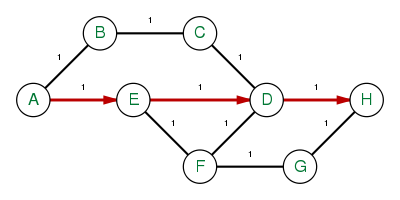
\includegraphics[]{bahdari_2.png}
\end{figure}
\item Zastąpić każdą krawędź w znalezionej ścieżce krawędzią skierowaną w przeciwną stronę oraz zmienić ich wagi na przeciwne (Rysunek 2);
\begin{figure}[H]
\caption{Zmiana kierunków krawędzi oraz znaków wag}
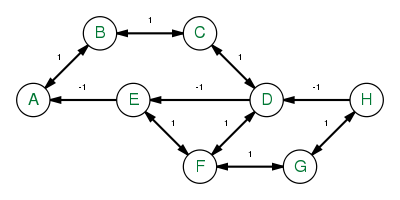
\includegraphics[]{bahdari_3.png}
\end{figure}
\item Dla tak zmodyfikowanego grafu ponownie znaleźć najkrótszą ścieżkę dla tej samej pary węzłów, używając zmodyfikowanego algorytmu Djjkstry (podrozdział 2.1.2) aby można było rozważać negatywne wagi krawędzi (Rysunek 3);
\begin{figure}[H]
\caption{Wynik działania zmodyfikowanego algorytmu Dijkstry}
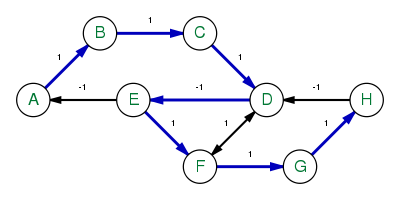
\includegraphics[]{bahdari_4.png}
\end{figure}
\item Stworzyć graf złożony z obu znalezionych ścieżek (wierzchołki ścieżek odpowiadają wierzchołkom z grafu macierzystego), w przypadku wykorzystania w drugiej ścieżce którychś z krawędzi otrzymanych po inwersji krawędzi ze ścieżki pierwszej te wykorzystane krawędzie i ich oryginały są usuwane z grafu (Rysunek 4 i 5)
\begin{figure}[H]
\caption{Graf złożony z obu znalezionych ścieżek}
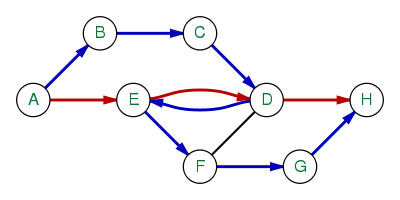
\includegraphics[]{bahdari_5.png}
\end{figure}
\begin{figure}[H]
\caption{Wynikowe ścieżki rozłączne krawędziowo}
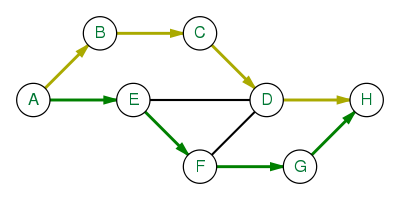
\includegraphics[]{bahdari_6.png}
\end{figure}
\item Otrzymujemy 2 rozłączne krawędziowo ścieżki w grafie, których suma wag jest najmniejsza spośród wszystkich ścieżek między tymi wierzchołkami (tak jak było w założeniach)
\end{itemize}
\subsubsection{Algorytm Dijkstry - szukanie najkrótszej ścieżki}
\tab
\begin{itemize}

\item Oznaczyć wszystkie wierzchołki jako nieodwiedzone, przypisać wierzchołkowi z którego szukamy najkrótszej ścieżki wartość 0, oznaczyć go jako wierzchołek obecny, wszystkim innym wierzchołkom przypisać wartość nieskończoną
\item Dla wszystkich nieodwiedzonych wierzchołków sąsiadujących z wierzchołkiem obecnym obliczyć wartość ich odległości od wierzchołka początkowego jako sumę wartości przypisanej wierzchołkowi obecnemu i wagi krawędzi prowadzącej z wierzchołka obecnego do wierzchołka dla którego obliczana jest odległość, następnie jeżeli obliczona wartość jest mniejsza od obecnie przypisanej danemu wierzchołkowi sąsiadującemu to podmieniamy tą wartość na nową
\item Oznaczamy obecny wierzchołek jako odwiedzony, po czym wybieramy spośród nieodwiedzonych wierzchołków ten który ma najmniejszą wartość, ustawiamy go jako obecny i powtarzamy punkt 2
\item Jeżeli wierzchołek docelowy został oznaczony jako odwiedzony albo najmniejsza przypisana wierzchołkowi nieodwiedzonemu wartość wynosi nieskończoność, to algorytm kończy działanie
\end{itemize}
Przy przypisywaniu wartości poszczególnym wierzchołkom można zapamiętywać wierzchołek z którego nadawana jest wartość i dzięki temu otrzymywać na koniec działania algorytmu najkrótszą drogę.

\subsubsection{Algorytm Bellmana-Forda}
\tab
Jest to zmodyfikowany algorytm Dijkstry, pozwalający na operacje na negatywnych wartościach wag krawędzi.
\begin{itemize}

\item Przypisać wierzchołkowi z którego szukamy najkrótszej ścieżki wartość 0, wszystkim innym wierzchołkom przypisać wartość nieskończoną
\item W pętli o N-1 (gdzie N - liczba wierzchołków) iteracjach dla każdej krawędzi porównujemy wartość przypisaną wierzchołkowi docelowemu krawędzi i sumę wagi krawędzi i wartości przypisanej do wierzchołka wejściowego krawędzi, po czym jeżeli suma jest niższa, podmieniamy na nią wartość przypisaną do wierzchołka docelowego
\item Jeżeli dla N-tej iteracji wciąż można poprawiać wartości przypisane, to w grafie istnieje cykl spowodowany negatywną wagą krawędzi, co skutkuje zakończeniem działania algorytmu bez poprawnego rozwiązania
\end{itemize}

Podobnie jak w algorytmie Dijkstry, dzięki śledzeniu skąd nadchodzi modyfikacja wartości wierzchołka można wyznaczyć szukaną ścieżkę do wierzchołka docelowego



\subsection{Wybór struktur danych}
\tab
W programie zostaną wykorzystane struktury danych z biblioteki standardowej języka C++. Dla algorytmu Dijkstry optymalnym rozwiązaniem do przechowywania wierzchołków jest $std::priority\_queue$. W pozostałych przypadkach wykorzystany będzie kontener $std::vector$ zawierający pojedyncze wielkości lub krotki.

\subsection{Projekty testów}
\tab
Testy programu będą obejmowały poprawność jego działania oraz uzyskiwaną wydajność. Poprawność będzie możliwa do zbadania w przypadku posiadania przez nas prawidłowych ścieżek referencyjnych do badanych grafów. W takim przypadku będzie można utworzyć skrypt uruchamiający program będący tematem niniejszego sprawozdania dla różnych grafów oraz porównujący uzyskiwane pliki wyjściowe z prawidłowymi, referencyjnymi wynikami.\\
\tab
Wydajność będzie badana dzięki pomiarowi czasu pracy procesora dla każdego wykonania programu. Aby test był jak najbardziej wiarygodny, utworzony zostanie skrypt uruchamiający program kilkanaście razy dla tego samego grafu oraz podający jako wynik najkrótszy czas z uzyskanych wyników.\\
\tab
Badanie i porównywanie złożoności obliczeniowej z teoretyczną będzie wykonywane dla wystarczająco długich ścieżek w grafach, gdyż poszukiwanie krótkich (w stosunku do najdłuższej ścieżki w grafie) ścieżek będzie dawało zaniżone wyniki.

\subsection{Założenia programu}
\tab
Program zostanie napisany w języku C++ ze względu na wysoką wydajność kodu wynikowego, oraz preferencje autorów niniejszego sprawozdania. Interfejs użytkownika nie będzie wykorzystywał biblioteki graficznej (wywołanie programu oraz jego obsługa będzie odbywała się z poziomu konsoli). Program będzie pozwalał na wczytanie pliku zawierającego badany graf poprzez podanie jego ścieżki w formie argumentu wywołania aplikacji. Kolejnymi dwoma argumentami wywołania będą nazwy wierzchołków dla których Użytkownik zechce znaleźć dwie najkrótsze sumarycznie ścieżki rozłączne krawędziowo. Ostatnim argumentem wywołania będzie ścieżka pliku wynikowego zawierającego dwie znalezione ścieżki zapisane w tym samym formacie co plik wejściowy. Na standardowe wyjście zostanie wypisany czas procesora wykorzystany podczas pracy algorytmu oraz uzyskana złożoność obliczeniowa. Dzięki temu będzie można utworzyć zewnętrzny, prosty skrypt (np. w języku Bash) pozwalający uśrednić czas działania i złożoność obliczeniową dla wielu przypadków.



\begin{thebibliography}{9}

\bibitem{surb}
  Suurballe, J. W.,
  \emph{Disjoint paths in a network}.
  Networks, 4, 1974, 125-145. 
\bibitem{bhan}
  Ramesh Bhandari,
  \emph{Survivable Networks: Algorithms for Diverse Routing}.
  Kluwer Academic Publishers, 1999 



\end{thebibliography}


\iffalse
\section{Tresc}
\subsection{Podpunkt pierwszy}
Plaszy!
\subsection{Wypunktowania}
To jest wypunktowanie:
\begin{itemize}
\item punkt
\item punkt
\item punkt
\end{itemize}
\subsection{Wyliczenie}
To jest wyliczenie:
\begin{enumerate}
\item pierwszy,
\item drugi,
\item trzeci.
\end{enumerate}
\subsection{Wykres}
Na Rysunku~\ref{fig:wykres} znajduje sie przykladowy wykres.
\begin{figure}[H]
%\includegraphics[width=\textwidth]{wykres}
\caption{Przykladowy wykres}
\label{fig:wykres}
\end{figure}
\subsection{Wzory}
\begin{equation}
2 + 2 = 4
\end{equation}
\begin{equation}
E = mc^2
\end{equation}
\begin{equation}
\left[- \frac{\hbar^2}{2M} + V(X) \right] \Psi(x)=  \mathcal{E} \Psi(x)
\end{equation}

\section{Podsumowanie}
\fi

\end{document}
